% Todo:

\documentclass[12pt]{article}
\usepackage{amsmath}	% for \genfrac
\usepackage[no-math]{fontspec}	% no-math option required for accents package
\usepackage{hyperref}
\usepackage{xeCJK}
%\setCJKmainfont{SimSun}
\setCJKmainfont[BoldFont=SimHei,ItalicFont=KaiTi]{SimSun}
% \setCJKsansfont{SimHei}
% \setCJKmonofont{SimKai}
% \usepackage{quattrocento}
% \usepackage{DejaVuSerif}
%\usepackage[sfdefault]{ClearSans} 
%\usepackage[defaultsans]{droidsans}
%\renewcommand*\familydefault{\sfdefault}
\usepackage{fontenc}
\usepackage[light]{merriweather}
% \setmainfont{Arial}

\usepackage{accents}		% for dots under Chinese for empahsis
\usepackage{cite}
\usepackage{graphicx}
\usepackage{float}
\usepackage{amsfonts}
\usepackage{amssymb}	% for \multimap
% \usepackage{stmaryrd}
\usepackage{color}
%\usepackage[square,numbers]{natbib}
%\nocopyright
%\usepackage{latexsym,amsmath,amssymb,graphicx,hyperref}
%\usepackage{times} % gives you a bit more space if needed
\usepackage{titlesec}		% change color of section headings
\usepackage{verbatim}		% enables to define {comment} blocks
% \usepackage[most]{tcolorbox}		% color box
\usepackage{tikz-cd}		% commutative diagrams
\usepackage{enumerate}

% Left and right angle brackets
\makeatletter
\newsavebox{\@brx}
\newcommand{\llangle}[1][]{\savebox{\@brx}{\(\m@th{#1\langle}\)}%
  \mathopen{\copy\@brx\kern-0.5\wd\@brx\usebox{\@brx}}}
\newcommand{\rrangle}[1][]{\savebox{\@brx}{\(\m@th{#1\rangle}\)}%
  \mathclose{\copy\@brx\kern-0.5\wd\@brx\usebox{\@brx}}}
\makeatother

% Make dots under Chinese characters for emphasis
\renewcommand{\d}[1]{$\underaccent{\scalebox{0.7}{\textbullet}}{\textrm{#1}}$}
\makeatletter\newcommand{\ds}[1]{\@tfor\next:=#1\do{\d{\next}}}\makeatother

\titleformat{\section}
{\color{blue}\normalfont\Large\bfseries}
{\color{blue}\thesection}{1em}{}
\titleformat{\subsection}
{\color{blue}\normalfont\large\bfseries}
{\color{blue}\thesubsection}{1em}{}

\renewcommand\abstractname{\textcolor{blue}{Abstract}}

\definecolor{LogicColor}{rgb}{0.4,0.1,0.4}  % Magenta
\definecolor{Hilight}{rgb}{0.9,0.9,0.8}  % yellow
\definecolor{grey}{rgb}{0.9,0.9,0.9}  % grey
% \definecolor{LogicColor}{rgb}{0,0,0}	% for black-and-white paper

\newcommand{\concept}[1]{\textbf{\textcolor{blue}{#1}}}

\newcommand{\english}[1]{\rmfamily \textit{``#1''}\rmfamily}
\newcommand{\formula}[1]{\textcolor{LogicColor}{#1}}

\newcommand{\hilight}[1]{\begin{tcolorbox}[breakable]#1\end{tcolorbox}}

\newcommand{\tab}{\hspace*{1cm}}
\newcommand{\dashh}{\textemdash~}

\newcommand*\sigmoid{\vcenter{\hbox{
\includegraphics{sigmoid.png}}}}
\newcommand*\sadface{
\includegraphics[scale=0.25]{face-sad.png}}
\newcommand*\smiley{
\includegraphics[scale=0.5]{smiley.jpg}}

\title{\textcolor{blue}{Genifer 5.3 theoretical notes}}
\author{YKY (甄景贤)}
%% \date{30 June 2015}
%% \institute{}

\overfullrule=1mm

\begin{document}

%\tab\tab\tab \parbox{9cm}{\textit{筌者所以在鱼,得鱼而忘筌;蹄者所以在兔,得兔而忘蹄;言者所以在意,得意而忘言。}}
% \vspace{-0.5cm}
%\begin{flushright}
%\textemdash\, 
%\textit{《庄子 $\cdot$ 外物》} \hspace*{2cm}
%\end{flushright}

% \sffamily

% {\let\newpage\relax\maketitle}

\maketitle
\setlength{\parindent}{0em}
\setlength{\parskip}{2.5ex plus0.5ex minus1.2ex}

\begin{abstract}
This is a completely new architecture: a long vector represents the cognitive state of the Reasoner, where a ``recurrent'' neural network acts on it to yield the new cognitive state.  This corresponds to a logical inference step in the classical paradigm.  A top-level reinforcement learner controls this Reasoner, having access to its cognitive states.
\end{abstract}

\setlength{\abovecaptionskip}{-10ex}
\setlength{\belowcaptionskip}{-18ex}

\setlength{\oddsidemargin}{1cm}
\setlength{\evensidemargin}{1cm}
\setlength{\textwidth}{14cm}

\linespread{1.2}

\section{Cognitive states}

As an example consider:
\begin{itemize}
\item It is 3:00AM in the morning
\item I am hungry
\item The refrigerator is empty
\item The MacDonald's downstairs is closed
\item .... etc
\end{itemize}
This is an example of my \textbf{cognitive state} that can be acted on to generate new conclusions.

In classical logic-based AI we have this dynamics:
\begin{figure}[H]
\centering
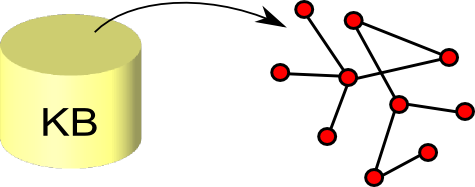
\includegraphics[scale=0.5]{classical-LBAI.png}
\end{figure}
where the KB (knowledge base) contains logical \textbf{facts} and \textbf{rules}.  \textit{Rules act on facts} to generate new \textbf{propositions} about the world.

In the new Genifer architecture, we introduce the \textbf{cognitive state vector} $K$ which is acted on by a \textbf{recurrent neural network} (RNN) \footnote{Recurrent here means a simple multi-layer feed-forward NN with its output fed back to its input, which is different from the standard meaning where hidden neurons have \textit{free} connections.} $D$:
\begin{figure}[H]
\centering
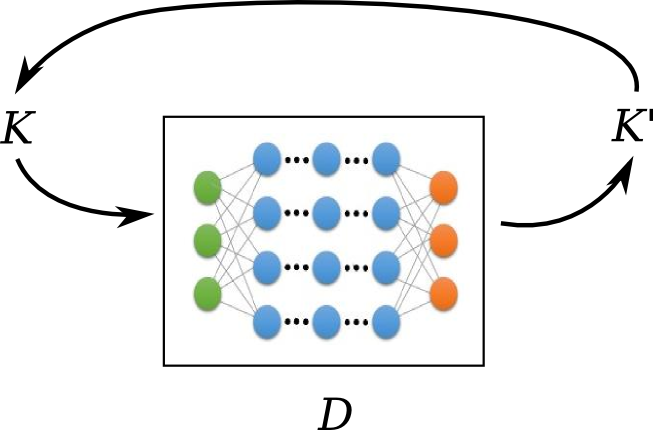
\includegraphics[scale=0.75]{reasoner-model.png}
\end{figure}
$K$ can be regarded as ``\textbf{working memory}'' in cognitive science.  $D$ stands for ``deduction'' in classical logic-based AI, but as we shall see it is more general than deduction.  The key point is the ability of $D$ to perform \textit{multi-step} inference operations on $K$.

\begin{figure}[H]
\centering
\colorbox{yellow}{\parbox{0.7\textwidth}{
\begin{tabular}{ccc}
facts in KB & $\Leftrightarrow$ & cognitive state vector $K$ \\
logic rules & $\Leftrightarrow$ & recurrent neural network \\
\end{tabular}
}}
\end{figure}

The cognitive state vector $K$ could be like this:
\begin{figure}[H]
\centering
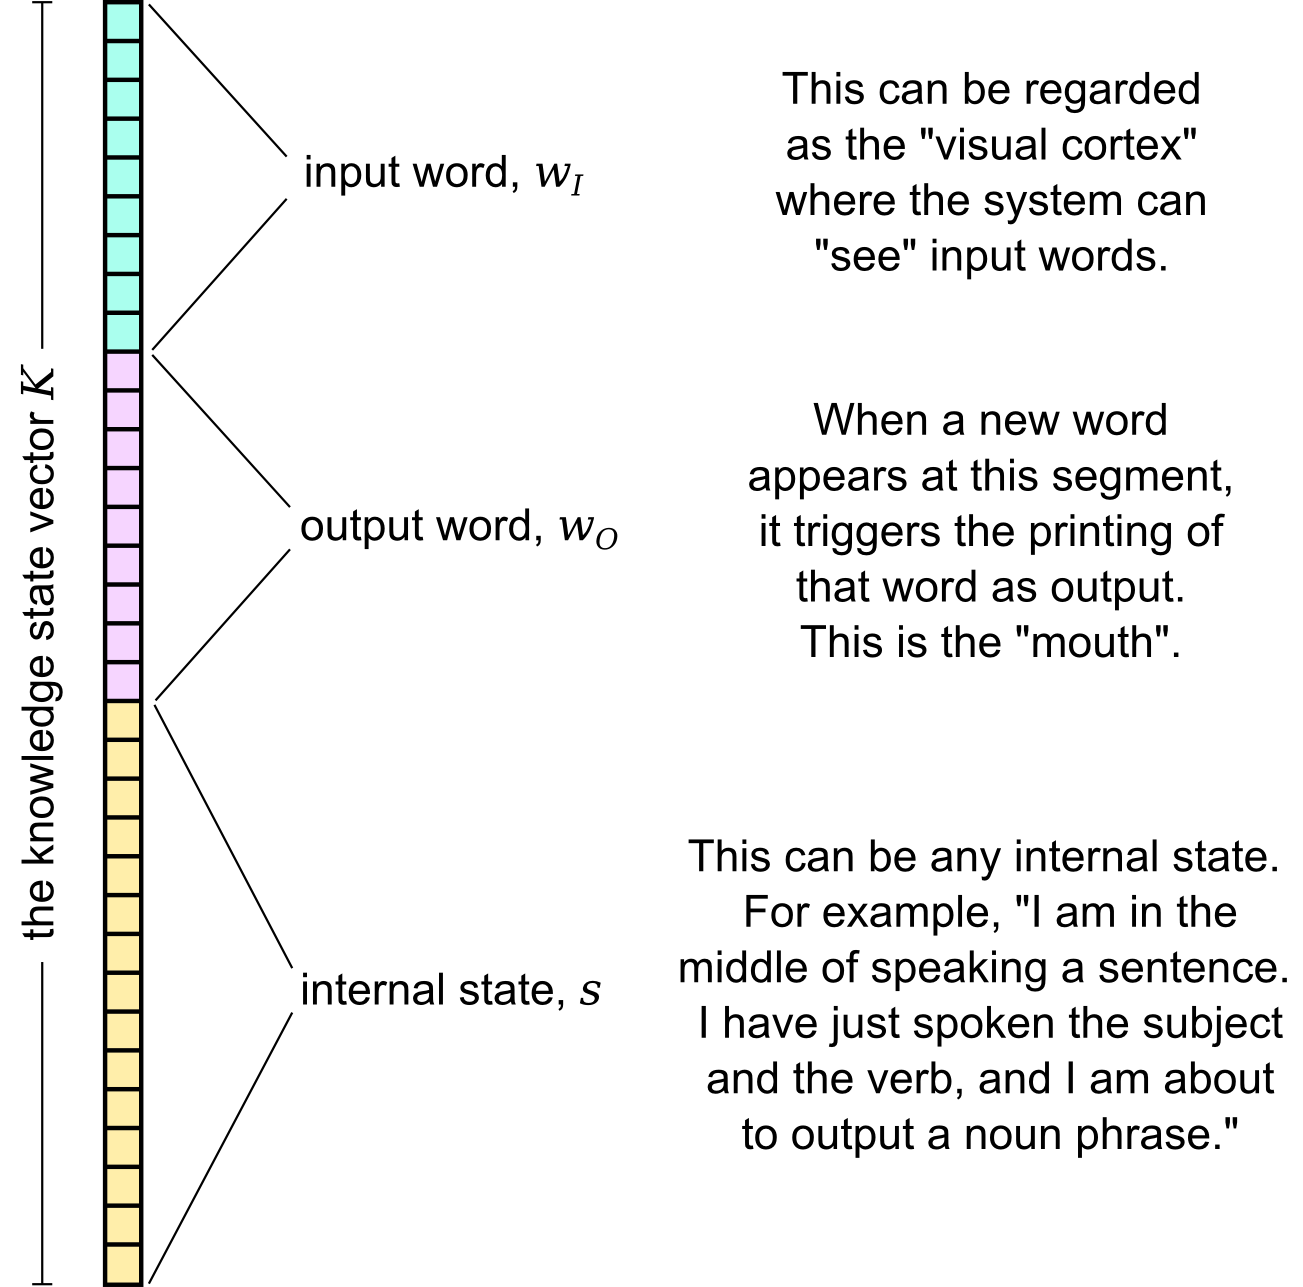
\includegraphics[scale=0.75]{internal-state-K.png}
\end{figure}

The general operation of Genifer could be like this:
\begin{center}
\begin{tikzcd}%[column sep=small]
\mbox{sentence input}\arrow[r,"\scalebox{1.3}{$\mathcal{L}$}"] & \mathbf{K} \arrow[r,"\scalebox{1.3}{$\mathcal{L}^{-1}$}"] \arrow[loop,"\scalebox{1.3}{$D$}",swap,looseness=4] & \mbox{sentence output}
% S\arrow{r} & K\arrow{r}\arrow{r}{loop,"D"} & S
\end{tikzcd}
\end{center}
where $\mathcal{L}$ is the ``\textbf{natural-language map}''.  As we shall see, $\mathcal{L}$ is not really needed.

The use of an RNN to act on the cognitive state vector is a radical departure from classical logic-based AI.  There is nothing in the new system that directly corresponds to propositions in classical logic.  For example, Genifer may believe that ``I should not be superstitious", but there may be nothing in the RNN or in $K$ that corresponds to the \textit{symbolic} representation of such a sentence.  If Genifer utters the sentence ``I should not be superstitious", it is \textit{generated} from the cognitive dynamics of the RNN.

Moreover, $D$ no longer needs to correspond to \textit{single} steps of logical inference.  Our formulation implicitly relaxed the requirement so that $D$ could be ``\textbf{fractional}'' or even ``\textbf{infinitesimal}'' inference steps.  The latter case might involve Lie groups or algebras, something I have not explored yet.

\section{Language map}

Genifer is not the first model that uses an RNN to model logical reasoning.  My friend Joseph Cheng showed me a paper from Facebook AI Research group \cite{Weston2015}, that proposed \textbf{Memory Networks} for Q \& A tasks.  It has a component $I$ = input feature map, responsible for parsing natural-language sentences into internal feature representations.

$\mathcal{L}$ turns NL sentences into internal representation of knowledge in $\mathbf{K}$, where $\mathbf{K} \ni K$ is the space of all cognitive states:
\begin{eqnarray}
\mathcal{L} :& \mathbf{S} & \rightarrow \mathbf{K} \nonumber \\
\mathcal{L} :& \mbox{sentence} & \mapsto K \nonumber
\end{eqnarray}
(Actually the sentence representation is just a part of $K$.)

\begin{center}
\begin{tikzcd}%[column sep=small]
\mbox{sentence input}\arrow[r,"\scalebox{1.3}{$\mathcal{L}$}"] & \mathbf{K} \arrow[r,"\scalebox{1.3}{$\mathcal{L}^{-1}$}"] \arrow[loop,"\scalebox{1.3}{$D$}",swap,looseness=4] & \mbox{sentence output}
\end{tikzcd}
\end{center}

Having this \textbf{language map} is very convenient, but it has a few problems:
\begin{itemize}

\item it requires NLP parsing, which is troublesome; better if we could avoid it

\item the map $\mathcal{L}$ basically \textit{fixed} the internal knowledge representation format.  But my intuition is that the knowledge representation should better be ``unknown'', it should be \textit{induced} through the learning process of $D$.

In traditional logic-based systems, $K$ = KB is a collection of logical propositions, $ K = \bigsqcup P_i $.  At that time, we tried to organize the KB hierarchically, so as to speed up searching and retrieval.  But I feel that if the structure of $\mathbf{K}$ is also the same, it would be ``too similar'' to the original setting, and everything is ``too orderly'', which may not be the best way to apply neural networks.

\item Natural langauge requires slow ``absorption'' or ``comprehension'', but this process is ignored in the Memory Network model.  Translation of NL sentences into logical form (ie, the internal representation) can almost be done \textit{instantaneous\-ly}.  But if we input the raw text of a \textit{World History} book to Genifer, and she translated it into internal representation within 1 second, can we say that Genifer has truly ``understood'' the content of the book?

\end{itemize}

\section{Slow comprehension}
% \label{language-comprehension}

Therefore $\mathcal{L}$ is not an ordinary map but a very complex \textit{process}.

The ``slow absorption'' of new input consists of these operations:
\begin{itemize}
\item \textbf{consequences} (find out all logical entailment of the new input, at least within $n$ steps of inference)
\item \textbf{consistency} (new beliefs do not contradict old ones)
\item \textbf{explanations} (new beliefs can be explained in terms of old ones)
\end{itemize}

The process of ``comprehension'' can be realized as the transformation of $K$ into a ``knowing'' state $K'$ after $n$ steps of inference:
\begin{center}
\begin{tikzcd}[row sep=tiny]
K \arrow[r, mapsto, "\scalebox{1.3}{$D^n$}"] & K'
\end{tikzcd}
\end{center}
% $$ K \stackrel{D^n}{\mapsto} K' $$
and we want $K'$ to possess the desired properties (consequence, coherence, explanation).  The question is how to test if $K'$ has such properties?  Particular difficulty stems from the fact that the representation of $K' \in \mathbf{K}$ is \textit{not transparent}.

To test the content of $K'$ we need a query $Q$:
\begin{center}
\begin{tikzcd}[row sep=tiny]
K \arrow[r, mapsto, "\scalebox{1.3}{$D^n$}"] & K' \stackrel{?}{\;=\;} Q
\end{tikzcd}
\end{center}

If we have $\mathcal{L}$, we can directly ask in natural language, via the query $Q = \mathcal{L}(\mbox{sentence})$, to test $K$.  In other words, the advantage of $\mathcal{L}$ is to allow \textit{direct access} to $K$, so that we can read out or write to the cognitive state.  But a simple $\mathcal{L}$ map does not exist in reality.

But all is not lost:  One advantage of a neural network is that it can simultaneously learn 2 processes, even if the 2 processes are \textit{inter-dependent}!  In \S\ref{sec:learning-to-listen-talk} we look at how to learn to listen and talk.

\section{Top-level architecture}

According to Richard Sutton, \textbf{reinforcement learning} (RL) should be the controlling module of an AI agent at the top level.  So we let the RL control the RNN (recurrent neural network):
\begin{center}
\fbox{\parbox[b][][t]{3.5em}{RL \\
\fbox{\parbox[c][][s]{2.5em}{RNN} }
} }
\end{center}

Or more detailedly:
\begin{figure}[H]
\centering
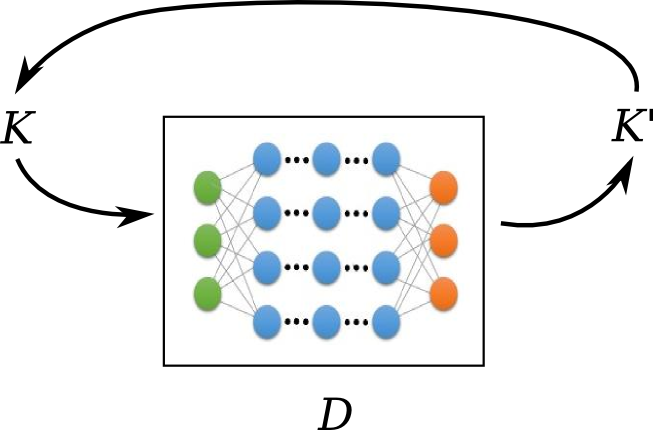
\includegraphics[scale=0.75]{genifer-model-0.png}
\end{figure}

We can think of the RNN as the RL's ``mental model'';  in other words, our RL has a more complex \textbf{world model} than traditional RL agents.

See my \href{http://geniferology.blogspot.hk/2015/05/what-is-reinforcement-learning.html}{blog post} for an introduction to reinforcement learning.

The remaining work is to define the 4 elements of RL: \textbf{states}, \textbf{actions}, \textbf{rewards}, \textbf{policy}.

\section{Unifying RL and RNN}

From the viewpoint of reinforcement learning, we aim to learn the \textbf{policy} function: \par
\begin{figure}[H]
\centering
\begin{tikzcd}[]
\mbox{policy : ~~state} \arrow[r, mapsto, "\scalebox{0.8}{action}"] & \mbox{state'}
\end{tikzcd}
\end{figure}
Where $K$ can be regarded as the \textbf{mental state}, and thus an \textbf{action} in RL is to turn $K$ into $K'$.

In our system, there are 2 pathways to act on $K$, via RNN and RL respectively: \par
\begin{figure}[H]
\centering
\begin{tikzcd}[column sep=huge]
& K'_1 \arrow[dd, dashed, no head, "\scalebox{1.3}{$\approx$}"] \\
K \arrow[ur, "\mbox{RL}"] \arrow[dr, "\mbox{RNN}"'] & \\
& K'_2
\end{tikzcd}
\end{figure}
In RL, the action $a$ acts on $K$, whereas in RNN, $D$ acts on $K$.

\textbf{Note}: RNN and RL are learning algorithms, and if they are both applied to the same problem, conflicts will necessarily arise, unless there is a way to combine them.

Assuming the learning is correct, $K'_1$ and $K'_2$ should be roughly the same \textemdash~ but this ignored the possibility that one path may take multiple steps to converge with the other path.  \footnote{This situation has been encountered in term rewriting systems (TRS):  If in a TRS any 2 different rewriting paths always converge to the same result, it is said to have the \textbf{Church-Rosser property}.  For example the $\lambda$-calculus invented by Church has this property.} 

Now I stipulate that $D$ be more ``refined'', that is to say, applying $D^n$ times may be equivalent to applying $a$ once:
\begin{figure}[H]
\centering
\begin{tikzcd}[column sep=huge]
& K'_1 \arrow[dd, dashed, no head, "\scalebox{1.3}{$\approx$}"] \\
K \arrow[ur, "\scalebox{1.3}{$a$}"] \arrow[dr, "{\scalebox{1.3}{$D^n$}}"'] & \\
& K'_2
\end{tikzcd}
\end{figure}
Using a different notation, $a$ is the \textbf{restriction} or \textbf{section} of $D^n$ at point $K$: $a = D^n|_K$.

Now the question is, do the RNN and RL paths have any \textit{essential} difference?
\begin{itemize}
\item Their internal \textbf{representations} are different:\\
\dashh RNN is a multi-layer neural network\\
\dashh RL's representation is $Q(\mbox{state},\mbox{action})$, although $Q$ could be approximated by a neural network as well.
\item RL learns through \textbf{rewards}, RNN learns from \textbf{errors}.  Thus RL has broader applicability, because not all questions have ``correct answers'' that could be measured by errors.  In RL we just need to praise Genifer whenever she displays good behavior.
\item The internal cognitive state $K$ exists because of RNN:  it is simply the vector input and output of the RNN.  Without this $K$, RL would be clueless as to what are its internal states.  It can be said that the RNN provides a \textit{machinery} for RL to control.
\end{itemize}

% programming needed:
% RNN: with special back-prop
% RL: approximate Q(K,a), using special NN that can find max also

% 整体来说,RL 可以操控的 actions 包括:
% \begin{enumerate}[\tab (A)]
% \item apply $K \stackrel{D}{\mapsto} K'$ \par
% 但注意: $K$ 是认知状态,$D$ 是对 $K$ 进行「合乎逻辑的推论」。 所以,无论发生什么事,我们都会将 $D$ 作用在 $K$ 上几次。 换句话说,$D$ 是\ds{必然}进行的动作,或者可以看成是在\ds{背景}下进行的运作,所以不需要用 RL 学习。 %RL 的用处是学习如何在很多 actions 之间选择最好的一个,所以 $D$ 不是 RL 需要学习的 action,它只是。

% \item 改写认知状态 $K \mapsto K'$ \par
% RL 的 actions (A) 是
% 在思考过程中改变 $K$ 的值。 例如我们得到一个局部结论,这个局部结论的状态不是最终答案,但也比什么都没有的效用更高。 改写 $K$ 的方法可以是: 例如 将 $K \mbox{ += } \delta K$,或者 「if $K \in$ 某 region,then $K \mbox{ += } \delta K $」。

% \item 学习: change $D$ \par

From the perspective of reinforcement learning, we could reward some results of multi-step inference: \par
\begin{figure}[H]
\centering
\begin{tikzcd}[row sep=tiny]
K_0 \arrow[r, mapsto, "\scalebox{1.3}{$a$}"] & K_\vdash \quad \updownarrow \bigstar
\end{tikzcd}
\end{figure}
$\updownarrow \bigstar$ means ``to give positive or negative rewards''.  We want to learn $a$ which is the action to be taken at state $K$.  The learning algorithm is based on the famous \textbf{Bellman optimality condition} (see next section).

Perhaps we should use RL to \textit{guide} the learning in RNN, as RNN is more fine-grained....

To combine the 2 learning approaches, we could use the technique of \textbf{interleaving}: for each step apply RL once, apply RNN $n$ times.

% 但 $D$ 本身是 RNN,它还可以透过 back-prop 进行学习,两者似乎是不同的。  Back-prop 是透过 $\frac{\partial}{\partial D}(\mbox{error})$ 的梯度来学习。

The learning in RNN may also involve \textbf{neurogenesis} (adding new neurons and connections), but I have not considered this aspect yet.

% RNN 的 $D$ 也是将 $K$ 变成 $K'$ 的作用:\par
%\begin{figure}[h]
%\centering
%\begin{tikzcd}[row sep=tiny]
%K \arrow[r, mapsto, "\scalebox{1.3}{$D$}"] & K'
%\end{tikzcd}
%\end{figure}
% $D$ 和 RL 的 actions 是不一样的。

There are 4 learning modes:
\begin{itemize}
\item learning to listen/talk
\item RL-based learning
\item inductive learning
\end{itemize}

\section{Bellman equation: the basis of RL}

Let's review the Bellman equation:
$$ U(S) = \max_a \{ R(S,a) + \gamma U(S') \}$$
where $U$ = utility, $R$ = reward, $\gamma$ = discount factor, $a$ = action, $S \stackrel{a}{\mapsto} S'$.  This is a recursive equation, expressing the relation between the optimal utility of the current state $U(A)$ and the optimal utility of the next state $U(S')$.

\begin{figure}[!h!t!b!p]
\begin{center}
\colorbox{grey}{\parbox{0.95\textwidth}{\setlength{\parskip}{2.5ex}
A bit of digression:  The Bellman equation has a \textbf{differential version}, known as the \textbf{Hamilton-Jacobi} equation, and nowadays the 2 can be unified as the Hamilton-Jacobi-Bellman equation.

Define a continuous version of ``utility'':
$$ U(x,t) = \min_u \{ \int_t^{t'} C(x,u)dt + U(x',t') \} $$
where $t$ is time, $u$ is a set of control parameters, $C$ is the \textbf{cost-rate} function:
$$ \int C dt = R = \mbox{reward} $$
This integral expresses the ``cost of the path'', whereas $U(x',t')$ is the ``cost at termination''.

The differential version is the Hamilton-Jacobi equation:
$$ \frac{d}{dt} U(x,t) = \min_u \{ C(x,u) + \langle \nabla U(x,t), f(x,u) \rangle \} $$
where $x$ must obey this dynamics:
$$ \dot{x}(t) = f(x(t),u(t)). $$

This equation is very close to the form of the \textbf{Schr\"{o}dinger} equation in quantum mechanics:
$$ i \hbar \frac{\partial}{\partial t} \Psi(x,t) = \left[ V(x,t) + \frac{-\hbar^2}{2\mu} \nabla^2 \right] \Psi(x,t). $$
$\Psi$ is analogous to our $U$ (perhaps it is something that nature wants to minimize?)
}}
\end{center}
\end{figure}

% 在思维过程中,除了结果以外,其他步骤是没有奖励的,所以 reward 只可以是一个微小的负常数(代表时间损耗):
% $$ R(S,a) \equiv -\epsilon \quad \mbox{(except for final states)}$$
% 在这情况下 Bellman 算法可能变到和 back-prop 差不多,甚至等价?

In our architecture, $K$ is the state, the action that acts on $K$ is always $D$ = RNN, but $D$ can change, $\mathbf{D} \ni D$ is the space of all the weights in the RNN.

$ U: \mathbf{S} \rightarrow \mathbb{R} $ is a function returning the \textbf{utility} of a mental states, which is \textit{unique} in reinforcement learning.  Yes! That is how RL learning is different from back-prop learning!  Some mental states could have higher utility than others, even though they are not the final answer state.  This corresponds to the feeling where we sometimes know our thinking is on the right track, despite that we have not reached final conclusion.

Perhaps we can use a separate neural network to approximate the utility function $U(\mbox{state})$ or $Q(\mbox{state},\mbox{action})$.

Algorithm for RL:  for each cycle, we apply $D$ (say, 10 times), and we get a new $K$.  Then we calculate:
$$ \mbox{action} = \arg\max_a Q(K,a) $$
which means we select the best action based on the optimal $Q$ value.  Note:  the fucntion $Q$ is learned using an external neural network, and then we need to find $Q$'s maximum, which involves \textit{another} optimization process (see appendix).  This needs to be very fast, and might be a bottleneck of the entire system.

As for the learning of $Q(K,a)$, the basic \textbf{update rule} is:
$$ Q(K,a) \;\mbox{ += }\; \eta (R(K,a) + \gamma \max_{\hat{a}} Q(K',\hat{a})) $$
where $\eta$ controls the learning speed.

\section{Learning to listen / talk}
\label{sec:learning-to-listen-talk}

Learning to listen/talk can be handled by RL:

\begin{enumerate}
\item learning to listen:
$$ \stackrel{\checkmark}{\mbox{input sentence}} \, \stackrel{?}{\longrightarrow} \, K \stackrel{{\color{red}\mbox{\footnotesize talk}}}{\longrightarrow} \, \mbox{output sentence} \, \approx_L \, \stackrel{\checkmark}{\mbox{testers}} $$
\item learning to talk:
$$ \stackrel{\checkmark}{\mbox{input sentence}} \, \stackrel{{\color{red}\mbox{\footnotesize listen}}}{\longrightarrow} \, K \, \stackrel{?}{\longrightarrow} \, \mbox{output sentence} \, \approx_L \, \stackrel{\checkmark}{\mbox{testers}} $$
\end{enumerate}

A $\checkmark$ means the data is known (= training set), ? is the map we want to learn, {\color{red}red} means inter-dependence (the listening and talking functions rely on each other during learning), $\approx_L$ is an \textit{external} function that compares the surface similarity of 2 natural-language sentences.  Testers are natural-language sentences used to test the correctness of listening and talking examples.

This seems to be more of a problem of designing training regimens, than of designing algorithms.

\begin{comment}
As to the learning algorithm, for example, assuming that K has been prepared,
\begin{figure}[H]
\centering
\begin{tikzcd}[row sep=tiny]
\stackrel{\checkmark}{K} \arrow[r, mapsto, "\scalebox{1.3}{$D^n$}"] & \mbox{output sentence} \quad \updownarrow \bigstar
\end{tikzcd}
\end{figure}
we can invoke the RL
\end{comment}

\section{Inductive learning}

For example:\\
\tab John is Chinese $\wedge$ John wears glasses \\
\tab Pete is Chinese $\wedge$ Pete wears glasses \\
\tab Mary is Chinese $\wedge$ Mary wears glasses \\
\tab Paul is Chinese $\wedge$ Paul wears glasses \\
\tab Conclusion: all Chinese people wear glasses \\
Expressed as a logical rule this is:
$$ \forall X. \; \mbox{Chinese}(X) \Rightarrow \mbox{wear-glasses}(X) $$
but this rule is implicitly encoded in $D$ by the RNN.  For example, if $K = \mbox{``Jane is Chinese''}$, then $D$ acting on $K$ would eventually result in $K' = \mbox{``Jane wears glasses''}$.

In other words, given $K_0$,$K^*$, learn $D$ such that:
$$ K_0 \stackrel{D}{\longrightarrow} .... \; K^* $$

If we have the map $\mathcal{L}$, we could use $K = \mathcal{L}(\mbox{NL sentence})$ to calculate $K_0$ and $K^*$, and this would be feasible.

Learning is done via back-prop, what we need is to start from $K_0$:
\begin{eqnarray}
K_0 \stackrel{D}{\longrightarrow} .... \; K_\vdash \nonumber \\
K_\vdash \ge K^* \nonumber
\end{eqnarray}
but this requires using the $\ge$ relation, discussed below.

The goal is to learn $D$, to minimize the error $\mathcal{E} = K_\vdash - K^*$.

The calculation of the gradient $\frac{\partial \mathcal{E}}{\partial W}$ should be feasible;  here $W$ is the weights of the RNN.

% But how do we calculate $\mathcal{E} = K_\vdash - K^*$?  There is a severe problem: we need to know the representation of $K^*$, but if $D$ is a \textit{black box}, the representation of $K^*$ would be \textit{opaque}.

\section{Querying}

Perhaps querying can be formulated as this problem:
\begin{eqnarray}
\mbox{solve}\quad\quad D^n(\mathbf{x}) & > & K^* \nonumber \\
K_0 & \ge & \mathbf{x} \nonumber
\end{eqnarray}
where $\mathbf{x}$ is the variable.  We require $>$ to exceed a threshold $\epsilon$.  This is an iterative equation, which seems hopeful.

If $D$ is \textbf{monotonous}, ie, $\forall \mathbf{x} \; D(\mathbf{x}) \ge \mathbf{x}$, this fact may be exploited to design faster algorithms.

\section{The \texorpdfstring{$\ge$}{>} relation}

$\ge$ is the \textbf{implication order} in logic (also similar to the \textbf{general-specific order}), it has 2 forms:
\begin{itemize}
\item all men are mortal $\ge$ Socrates is mortal
\item all men are mortal $\ge$ (all men are mortal $\wedge$ the moon is round)
\end{itemize}

In (topological) vector space theory, we can define a relation $\mathbf{v}_1 \ge \mathbf{v}_2$ between vectors, by selecting an arbitrary \textbf{cone} $C$:
$$ \mathbf{v}_1 \ge \mathbf{v}_2 \Leftrightarrow (\mathbf{v}_1 - \mathbf{v}_2) \in C $$
For example, on the 2D plane, $C$ could be the upper-right quadrant.

I am considering:  Can we just arbitrarily select a cone in the space $\mathbf{K}$ to define $\ge$, and then let the RNN learn the logical structure of $\ge$ itself (for example, animals $\ge $ cats, $A \ge A \wedge B$, etc)?

\setlength{\emergencystretch}{10pt}
\section*{Appendix: Finding maximum in a back-prop NN}

\textbf{Problem statement}:  We have used back-prop to train a neural network to approximate $Q(K,a)$.  But we don't have the explicit form of Q;  Q is realized \textit{implicitly} in the NN.  Now we need to find $\arg\max_a Q(K,a)$.

We can use \textbf{gradient descent} to find the (local) maxima, and repeat this over randomly-chosen starting points.  After many trials the result will approach global maximum.

The gradient descent \textbf{update rule} is:
$$ x^{k+1} = x^k - \eta \nabla y(x^k). $$

This process is quite similar to back-prop, with the difference that back-prop uses the gradient $\frac{\partial \mathcal{E}}{\partial W}$ whereas here we use the gradient $\frac{\partial y}{\partial x}$.

For each layer,
$$ y_j = \sigmoid( \sum W_{ji} x_i ) $$
and the overall output is:
$$ y = y_J \circ y_{J-1} \circ .... \, y_0 (x). $$
$J$ is the number of hidden layers.

We then calculate
$$ \nabla y = \left[ \frac{\partial y}{\partial x_l} \right] =
\frac{\partial y_J}{\partial y_{J-1}}
\frac{\partial y_{J-1}}{\partial y_{J-2}} .... \,
\frac{\partial y_0}{\partial x_l} $$
% $$ =
% \frac{\partial y_J}{\partial y_{J-1}}(y_{J-1})
% \frac{\partial y_{J-1}}{\partial y_{J-2}}(y_{J-2}) .... \,
% \frac{\partial y_1}{\partial y_0}(y_0)
% \frac{\partial y_0}{\partial x}(x). $$
At each step, we move a small amount in this direction.  But the above direct calculation of $\nabla y$ seems very complicated.  An alternative is to use \textbf{numerical differentiation}.

%%%%%%%%%%%%%%%%%%%%%%%%%%%%%%%%%%%%%%%%%%%%%%%%%%%%%%%%%%%%%%%%%%%%%%%%
% {\color{red}\rule{10cm}{2pt}}

\begin{comment}
%===========================================================================


%===========================================================================
\end{comment} 

\bibliographystyle{plain} % or number or aaai ...
\bibliography{AGI-book}

\end{document}
